\documentclass{article}
\usepackage[margin=.9in, bindingoffset=.2in, letterpaper]{geometry}
\usepackage{amsthm,amsmath,amsfonts}
\usepackage{amssymb,latexsym,amscd}
\usepackage{mathrsfs}
\usepackage[all,cmtip]{xy} 
%\usepackage{diagxy}
\usepackage{tikz}
\usetikzlibrary{calc}
\usepackage{tikz-cd}
\usepackage[hidelinks]{hyperref}
\usepackage{bookmark}
\usepackage{comment}
%\usepackage{showlabels}
%\usepackage{showkeys}
\usepackage{setspace}
\usepackage{bbm}
\usepackage{bm}
\usepackage{epstopdf}
\usepackage{stmaryrd}
\usepackage{enumerate}
\usepackage[mathscr]{euscript}
\usepackage{cleveref}
\hypersetup{pageanchor=false}
% \usepackage[noadjust]{cite}
\numberwithin{equation}{section}

\usepackage{dynkin-diagrams}
\usepackage{xspace}
%-----------------------------------------------------------------

\usepackage{datetime}
\renewcommand{\dateseparator}{-}
\renewcommand{\today}{\the\year \dateseparator \twodigit\month
	\dateseparator \twodigit\day}


\usepackage[natbib=true,url=false]{biblatex}
\addbibresource{main.bib}
\renewbibmacro{in:}{}
%-----------------------------------------------------------------

\DeclareMathOperator{\Id}{Id} 
\DeclareMathOperator{\Real}{Re}
\DeclareMathOperator{\Imaginary}{Im}
\DeclareMathOperator{\Tr}{Tr}
\DeclareMathOperator{\sgn}{sgn}
\DeclareMathOperator{\b|}{\boldsymbol{|}}
\DeclareMathOperator{\Var}{Var}
\DeclareMathOperator{\semicircle}{sc}
\DeclareMathOperator{\sign}{sign}


\DeclareMathOperator{\cone}{cone}
\DeclareMathOperator{\spn}{span}

% \DeclareMathOperator{\udim}{\,\underline{\!dim\!}\,}
\newcommand{\udim}{\operatorname{\underline{dim}}}
\DeclareMathOperator{\Spec}{Spec}


%-----------------------------------------------------------------
\DeclareFontFamily{U}{wncy}{}
\DeclareFontShape{U}{wncy}{m}{n}{<->wncyr10}{}
\DeclareSymbolFont{mcy}{U}{wncy}{m}{n}
\DeclareMathSymbol{\Sha}{\mathord}{mcy}{"58} 
\DeclareMathSymbol{\El}{\mathord}{mcy}{"4C} 
\DeclareMathSymbol{\Er}{\mathord}{mcy}{"52} 

\renewcommand{\aa}{\mathfrak{a}}
\renewcommand{\AA}{\mathbb{A}}
\newcommand{\BB}{\mathbb{B}}
\newcommand{\CC}{\mathbb{C}}
\newcommand{\DD}{\mathbb{D}}
\newcommand{\EE}{\mathbb{E}}
\newcommand{\FF}{\mathbb{F}}
\newcommand{\GG}{\mathbb{G}}
\newcommand{\HH}{\mathbb{H}}
\newcommand{\II}{\mathbb{I}}
\newcommand{\JJ}{\mathbb{J}}
\newcommand{\KK}{\mathbb{K}}
\newcommand{\LL}{\mathbb{L}}
\newcommand{\MM}{\mathbb{M}}
\newcommand{\NN}{\mathbb{N}}
\newcommand{\OO}{\mathbb{O}}
\newcommand{\PP}{\mathbb{P}}
\newcommand{\QQ}{\mathbb{Q}}
\newcommand{\RR}{\mathbb{R}}
\renewcommand{\SS}{\mathbb{S}}
\newcommand{\TT}{\mathbb{T}}
\newcommand{\UU}{\mathbb{U}}
\newcommand{\VV}{\mathbb{V}}
\newcommand{\WW}{\mathbb{W}}
\newcommand{\XX}{\mathbb{X}}
\newcommand{\YY}{\mathbb{Y}}
\newcommand{\ZZ}{\mathbb{Z}}
% \newcommand{\kk}{\Bbbk}

\newcommand{\cA}{\mathcal{A}}
\newcommand{\cB}{\mathcal{B}}
\newcommand{\cC}{\mathcal{C}}
\newcommand{\cD}{\mathcal{D}}
\newcommand{\cE}{\mathcal{E}}
\newcommand{\cF}{\mathcal{F}}
\newcommand{\cG}{\mathcal{G}}
\newcommand{\cH}{\mathcal{H}}
\newcommand{\cI}{\mathcal{I}}
\newcommand{\cJ}{\mathcal{J}}
\newcommand{\cK}{\mathcal{K}}
\newcommand{\cL}{\mathcal{L}}
\newcommand{\cM}{\mathcal{M}}
\newcommand{\cN}{\mathcal{N}}
\newcommand{\cO}{\mathcal{O}}
\newcommand{\cP}{\mathcal{P}}
\newcommand{\cQ}{\mathcal{Q}}
\newcommand{\cR}{\mathcal{R}}
\newcommand{\cS}{\mathcal{S}}
\newcommand{\cT}{\mathcal{T}}
\newcommand{\cU}{\mathcal{U}}
\newcommand{\cV}{\mathcal{V}}
\newcommand{\cW}{\mathcal{W}}
\newcommand{\cX}{\mathcal{X}}
\newcommand{\cY}{\mathcal{Y}}
\newcommand{\cZ}{\mathcal{Z}}

\newcommand{\tA}{\widetilde{A}}
\newcommand{\tB}{\widetilde{B}}
\newcommand{\tC}{\widetilde{C}}
\newcommand{\tD}{\widetilde{D}}
\newcommand{\tE}{\widetilde{E}}
\newcommand{\tF}{\widetilde{F}}
\newcommand{\tG}{\widetilde{G}}
\newcommand{\tS}{\widetilde{S}}
\newcommand{\tT}{\widetilde{T}}
\newcommand{\te}{\widetilde{e}}
\newcommand{\tpi}{\widetilde{\pi}}
\newcommand{\tH}{\widetilde{H}}
\newcommand{\tN}{\widetilde{N}}
\newcommand{\talpha}{\widetilde{\alpha}}

\newcommand{\sL}{\mathsf{L}}
\newcommand{\tR}{\widetilde{R}}

\newcommand{\newword}[1]{\textbf{#1}}

\newcommand{\GL}{\mathrm{GL}}

\newcommand{\be}{\mathbf{e}}
\newcommand{\bR}{\mathbf{R}}
\newcommand{\tbe}{\widetilde{\mathbf{e}}}

% \renewcommand{\aa}{{\mathfrak{a}}} % watch out in bibliography
% \newcommand{\bb}{{\mathfrak{b}}}
\newcommand{\taa}{{\widetilde{\mathfrak{a}}}} % watch out in bibliography
\newcommand{\tbb}{\widetilde{\mathfrak{b}}}

\newcommand{\aug}{{\mathrm{aug}}}
\newcommand{\taug}{\tT_{\mathrm{aug}}}

\newcommand{\rind}[1]{\mathopen{\boldsymbol{(}}#1\mathclose{\boldsymbol{)}}}%{(\widetilde{#1})}

\newcommand{\LowerArcs}{\mathsf{LowerArcs}}
\newcommand{\UpperArcs}{\mathsf{UpperArcs}}
\newcommand{\tLowerArcs}{\widetilde{\mathsf{LowerArcs}}}
\newcommand{\tUpperArcs}{\widetilde{\mathsf{UpperArcs}}}
\newcommand{\LowerWalls}{\mathsf{LowerWalls}}
\newcommand{\UpperWalls}{\mathsf{UpperWalls}}

\newcommand{\JIrrc}{\mathsf{JIrr}^c}
\newcommand{\MIrrc}{\mathsf{MIrr}^c}
\newcommand{\JI}{cJI\xspace}
\newcommand{\JIs}{cJIs\xspace}
\newcommand{\Arcs}{\mathsf{Arcs}}

\newcommand{\Tot}{\mathrm{Tot}}
\newcommand{\TTot}{\mathrm{TTot}}
\newcommand{\WO}{\mathsf{WO}}
\newcommand{\EWO}{\mathsf{EWO}}
\newcommand{\Dyer}{\mathsf{Dyer}}
\newcommand{\Contr}{\operatorname{\mathsf{Contr}}}

% \newcommand{\rind}[1]{\mathopen{\boldsymbol{(}}#1\mathclose{\boldsymbol{)}}}
\newcommand{\precdot}{\prec\mathrel{\mkern-5mu}\mathrel{\cdot}}


%----------------------------------------

\newtheorem{theorem}{Theorem}[section]
\newtheorem{proposition}[theorem]{Proposition}
\newtheorem{lemma}[theorem]{Lemma}
\newtheorem{corollary}[theorem]{Corollary}
\newtheorem{conjecture}[theorem]{Conjecture}
\crefname{conjecture}{Conjecture}{Conjectures}
\newtheorem{question}[theorem]{Question}
\newtheorem{problem}[theorem]{Problem}
\theoremstyle{remark}
\newtheorem{remark}[theorem]{Remark}
\newtheorem{example}[theorem]{Example}
\theoremstyle{definition}
\newtheorem{definition}[theorem]{Definition}

\newcommand{\threepartdef}[6]
{
	\left\{
	\begin{array}{lll}
		#1 & \mbox{if } #2 \\
		#3 & \mbox{if } #4 \\
		#5 & \mbox{otherwise.} #6
	\end{array}
	\right.
}

\newcommand{\kk}{\mathbbm{k}}
\newcommand{\Tors}{\mathsf{Tors}}
\newcommand{\Tam}{\mathsf{Tam}}
\newcommand{\OEG}{\mathsf{OEG}}

\title{Bruhat order and applications: Lecture 1}
\author{Grant T. Barkley}
\date{}

\begin{document}
	\maketitle
	
	This will be a story about certain groups, called Coxeter groups. These are groups that are generated from the reflective symmetries of various objects, and play a key role in many areas of algebra and geometry. Here is a list of some areas where Coxeter groups play a key role:
	\begin{itemize}
		\item Lie groups and Lie algebras
		\item Finite simple groups
		\item Uniform polytopes
		\item Lattices
		\item Incidence geometry (in particular, Schubert calculus)
		\item Quiver representations
		\item Invariant theory
		\item Braid groups
	\end{itemize} 
	
	The most familiar examples of Coxeter groups are the symmetric group $S_n$ and the dihedral groups $I_2(m)$ (more commonly denoted $D_{2m}$, although we will avoid that notation). How are these built from reflective symmetries? The dihedral group $I_2(m)$ is generated by the reflective symmetries of a regular $m$-gon. The symmetric group $S_n$ is generated from the reflective symmetries of an $(n-1)$-simplex.
	
	
	
	\section{The symmetric group}
	Let's briefly recall some conventions for working with the symmetric group. Let $[n]$ denote the set $\{1,2,\ldots, n\}$.
	\begin{definition}
		The \newword{symmetric group} $S_n$ is the group of bijections
		\[ \pi : [n] \to [n], \]
		where multiplication is given by composition of functions. Elements of $S_n$ are called \newword{permutations}.
	\end{definition}
	It is convenient to encode permutations using shorthand. The \newword{one-line notation} of a permutation $\pi$ is the following string of digits:
	\[ \pi(1)\pi(2)\cdots \pi(n). \]
	So, for example, there are two permutations of $[2]$, and their one-line notations are $12$ and $21$. The identity element in $S_n$ has one-line notation $123\cdots n$. The product of the permutations $213$ and $132$ is
	\[ 213 \cdot 132 = 231. \]
	
	Another useful way of encoding a permutation is using \newword{cycle notation}. A \newword{cycle} is a permutation which permutes some subset of $[n]$ in a cyclic order (such as sending $2$ to $4$, sending $4$ to $3$, sending $3$ to $5$, and sending $5$ back to $2$), and which fixes the remaining elements. We encode a cycle by writing the permuted numbers in their cyclic order and wrapping it with parentheses. For example, the cycle just mentioned is denoted $(2435)$. We could also write this as $(4352)$ or $(3524)$. We might also write $(2,4,3,5)$ with commas for clarity, but the meaning is the same. The most important cycles for us will be the \newword{transpositions}, which are the $2$-cycles. There are $\binom{n}{2}$ many transpositions in $S_n$. In $S_3$, the transpositions are $(12), (23),$ and $(13)$.
	
	Because transpositions will be so important for us, it is good to be aware of what multiplying by a transposition does to the one-line notation of a permutation. Let $\pi$ be a permutation and let $a<b$ be elements of $[n]$. Then right-multiplying by the transposition $(a,b)$ swaps the entries in positions $a$ and $b$: 
	\[  \textcolor{red}{35}241\cdot (1,2) = \textcolor{red}{53}241   \qquad\text{and}\qquad 3\textcolor{red}{5}2\textcolor{red}{4}1 \cdot (2,4) =  3\textcolor{red}{4}2\textcolor{red}{5}1. \]
	In contrast,  \emph{left-}multiplying swaps the \emph{values} $a$ and $b$:
	\[  (1,2) \cdot 35\textcolor{red}{2}4\textcolor{red}{1} =  35\textcolor{red}{1}4\textcolor{red}{2} \qquad\text{and}\qquad (2,4)\cdot 35\textcolor{red}{24}1 = 35\textcolor{red}{42}1. \]
	We will use these operations quite a bit.
	
	\section{Coxeter groups}
	
	We will define Coxeter groups at the end of the section. But it will be useful to discuss some features of a Coxeter group before we do so. 
	
	\subsection{Simple reflections}
	Every Coxeter group $W$ is equipped with a distinguished subset called $S$. The choice of $S\subseteq W$ is part of the data of a Coxeter group, like the choice of a multiplication operator is part of the data of a group. The elements of $S$ are called \newword{simple reflections} (or \newword{simple generators}); the definition of a Coxeter group requires them to generate $W$. Additionally, the elements of $S$ are required to have order $2$: if $s\in S$, then $s^2=e$ (and $s\neq e$). The number of simple generators is the \newword{rank} of $W$.
	
	The standard Coxeter group structure on $S_n$ uses the set $S = \{(1,2), (2,3), \ldots, (n-1,n)   \}$. For shorthand, we usually write $s_i = (i,i+1)$, so that $S = \{s_1,s_2,\ldots, s_{n-1}\}$. For the symmetric group, the elements of $S$ are also called \newword{simple transpositions}. One can check that the simple transpositions have order $2$ and generate $S_n$. The rank of $S_n$ is $n-1$.
	
	Because the elements in $S$ generate $W$, by definition, each element $w\in W$ can be written as a product $s_{i_1}s_{i_2}\cdots s_{i_k}$. Such a product is called a \newword{word} or \newword{expression} for $w$. The \newword{length} of the word $s_{i_1}\cdots s_{i_k}$ is $k$, the total number of generators used in the word. Words can have different lengths; here are two words for $312$:
	\[  312 = s_1s_2s_1s_2 = s_2s_1. \]
	
	The following definition is extremely important.
	\begin{definition}
		Let $W$ be a Coxeter group and let $w\in W$. The \newword{length} of $w$ is the minimum length of any word for $w$, and is denoted $\ell(w)$. A word for $w$ which has length $\ell(w)$ is called a \newword{reduced word}. 
	\end{definition}
	
	
	The length of $312$ is $2$, and $s_2s_1$ is a reduced word for $312$. The word $s_1s_2s_1s_2$ is not reduced. The permutation $321$ has two reduced words: $s_1s_2s_1$ and $s_2s_1s_2$, so reduced words are not unique. It is not obvious from the definition how one would compute $\ell(w)$ from the one-line notation, but we will shortly see that a property of Coxeter groups will make it easier.
	
%	Given a word $s_{i_1}\cdots s_{i_k}$ and an index $j$, we write $s_{i_1}\cdots \widehat s_{i_j} \cdots s_{i_k}$ to denote the word that results from deleting the $j$th letter from the original word. For example, $s_1s_2\widehat s_1 s_2 = s_1s_2s_2$. 
	
%	We are now ready to state the defining property of Coxeter groups (our first of several equivalent definitions).
%	
%	\begin{definition}[Exchange property]
%		Let $W$ be a group and let $S\subseteq W$ be a generating set of order-$2$ elements. Then $(W,S)$ is a \newword{Coxeter system} if, for any reduced word $w=s_{i_1}\cdots s_{i_k}$ and any $s\in S$ such that $\ell(sw)<\ell(w)$, there exists an index $j$ such that 
%		\[ sw = s_{i_1}\cdots \widehat s_{i_j} \cdots s_{i_k}. \]
%		In this case, we say that $W$, equipped with the simple reflections $S$, is a \newword{Coxeter group}. 
%	\end{definition} 
%	
	
	\subsection{Reflections}
	\newcommand{\inv}{\operatorname{inv}}
	In this section we will introduce the abstract notion of a reflection element in a Coxeter group. Later we will see that these abstract group elements actually correspond to honest-to-goodness reflections in a geometric setting.
	
	\begin{definition}
		Let $W$ be a Coxeter group with simple reflections $S$. An element $t\in W$ is called a \newword{reflection} if $t = wsw^{-1}$ for some $w\in W$ and $s\in S$. The set of reflections in $W$ is
		\[ T\coloneqq \{wsw^{-1} \mid w\in W, ~s\in S\}. \]
	\end{definition}
	
	In the symmetric group $S_n$, the reflections are exactly the transpositions. Hence $|T|=\binom{n}{2}$. It is sometimes useful to observe that an element of $W$ is a reflection if and only if it has an odd-length palindromic word, such as $s_1s_2s_3s_2s_1$. 
	The motivation for calling the elements of $T$ reflections will not be clear until we see some geometry, but we can find some applications right away. The idea is that reflections are the ``directions'' via which you can make a reduced word smaller. 
	
	\begin{definition}
		A (left) \newword{inversion} of $w\in W$ is a reflection $t\in T$ such that $\ell(tw) < \ell(w)$. The set of inversions of $w$ is denoted $\inv(w)$.  
		A (right) \newword{descent} of $w\in W$ is a simple reflection $s\in S$ such that $\ell(ws)<\ell(w)$. 
	\end{definition}
	
	If we are given a reduced word for $w$, then it is easy to write down a list of $\ell(w)$ many inversions of $w$. Let's say the reduced word is $s_{i_1}s_{i_2}\cdots s_{i_k}$. Then 
	\begin{align*}
		s_{i_1} \cdot w &=  \phantom{s_{i_1}}s_{i_2}s_{i_3}s_{i_4} \cdots s_{i_{k-1}}s_{i_k} \\
		s_{i_1}s_{i_2}s_{i_1} \cdot w &= s_{i_1}\phantom{s_{i_2}} s_{i_3}s_{i_4}\cdots s_{i_{k-1}}s_{i_k} \\ 
		s_{i_1}s_{i_2}s_{i_3}s_{i_2}s_{i_1} \cdot w &=s_{i_1} s_{i_2}\phantom{s_{i_3}}s_{i_4}\cdots s_{i_{k-1}}s_{i_k} \\
		\vdots\\ 
		s_{i_1}\cdots s_{i_{k-1}}s_{i_k}s_{i_{k-1}}\cdots s_{i_1} \cdot w &= s_{i_1} s_{i_2}s_{i_3}s_{i_4}\cdots s_{i_{k-1}}\phantom{s_{i_k}}.
	\end{align*}
	So multiplying $w$ by one of the elements on the left produces a (not necessarily reduced) word of length $k-1$, and thus an element of $W$ with length at most $k-1$. The elements on the left are all reflections, and it is not hard to show that they are all distinct. So a reduced word for $w$ gives a way to list $\ell(w)$ many inversions of $w$. Are these all of the inversions of $w$? Equivalently, is the number of inversions of $w$ equal to $\ell(w)$? The answer turns out to be yes, and this fact is so important that it actually gives a way of defining Coxeter groups. (There are many equivalent ways to define Coxeter groups, so this may not be the definition you have seen.)
	
	\begin{definition}
		Let $W$ be a group, and let $S\subseteq W$ be a generating set for $W$ so that every element of $S$ has order $2$. Define the set $T\coloneqq \{wsw^{-1}\mid w\in W,~s\in S\}$. Then $(W,S)$ is a \newword{Coxeter system} if, for all $w\in W$,
		\[ |\{t\in T \mid \ell(tw) < \ell(w) \}| = \ell(w). \]
		In this case, we say that $W$, equipped with the simple reflections $S$, is a \newword{Coxeter group}. 
	\end{definition}
	
	Let us test this definition by proving that $S_n$ is a Coxeter group. Along the way, we will characterize the inversions and descents in $S_n$. In the characterization, we will discuss the condition $\pi^{-1}(b)<\pi^{-1}(a)$. You don't need to compute $\pi^{-1}$ to understand this condition; all it means is that $b$ appears somewhere to the left of $a$ in the one-line notation of $\pi$. (This is because $\pi^{-1}(b)$ is the position of $b$ in the one-line notation of $\pi$, and similarly for $a$.)
	
	\begin{theorem}
		The following hold for a permutation $\pi \in S_n$:
		\begin{itemize}
		\item[(a)] The inversion set satisfies \[ \inv(\pi) = \{ (a,b) \mid 1\leq a < b \leq n\text{ and $ \pi^{-1}(b)<\pi^{-1}(a)$} \}; \]
		\item[(b)] $|\inv(\pi)|= \ell(\pi)$;
		\item[(c)]  The simple reflection $s_i$ is a descent of $\pi$ if and only if $\pi(i)>\pi(i+1)$.
		\end{itemize}
		Hence the symmetric group $S_n$, equipped with its generating set $S=\{s_1,\ldots,s_{n-1}\}$, is a Coxeter group.
	\end{theorem}
	\begin{proof}
		We will use induction on $\ell(\pi)$ to prove (a) and (b). If $\ell(\pi)=0$, then $\pi=e$. Since $e$ has no inversions, (b) holds for $e$. Since there are no pairs $(a,b)$ that appear out of order in $e$, (a) holds for $e$. 
		
		Now assume instead that $\ell(\pi)>0$ and that we know (a) and (b) for all permutations $\pi'$ with $\ell(\pi')<\ell(\pi)$. Let $s_i$ be a descent of $\pi$. Let $\pi'=\pi\cdot s_i$, so that $\ell(\pi')=\ell(\pi)-1$. Then by induction, we know (a) and (b) hold for $\pi'$. 
		
		Observe that right-multiplying $\pi'$ by $s_i$ causes the entries in positions $i$ and $i+1$ to swap. Since we know this raises the length of $\pi'$, that means $(\pi'(i),\pi'(i+1))$ is not an inversion of $\pi'$. Then property (a) for $\pi'$ implies that $\pi'(i) < \pi'(i+1)$. Hence $\pi(i)>\pi(i+1)$.  We will prove that
		\[ \inv(\pi) = \inv(\pi') \cup \{ (\pi(i), \pi(i+1)) \}. \]
		The right-hand side has size $\ell(\pi)$ (using property (b) for $\pi'$). Moreover it is not hard to see that the pairs of integers that are out of order in $\pi$ are exactly those that are out of order in $\pi'$, along with $(\pi(i),\pi(i+1))$. Hence proving the equality will prove both (a) and (b).
		
		Let $s_{i_1}\ldots s_{i_{k-1}}$ be a reduced word for $\pi'$. Then $s_{i_1}\cdots s_{i_{k-1}}s_i$ is a reduced word for $\pi$. We know from property (b) for $\pi'$ that any $t\in \inv(\pi')$ is equal to $s_{i_1}\cdots s_{i_j}s_{i_{j-1}}\cdots s_{i_1}$ for some $j$. Hence $t$ is also an inversion of $\pi$. This proves that $\inv(\pi')\cup \{(\pi(i),\pi(i+1))\}\subseteq \inv(\pi)$, since we already observed that $(\pi(i),\pi(i+1))\in \inv(\pi)$. Conversely, let $1\leq a < b \leq n$ and assume that $(a,b)\in \inv(\pi)$. Then $\ell((a,b)\cdot \pi)<\ell(\pi)$, so we inductively know property (a) holds for $(a,b)\cdot \pi$. We learn that $a$ appears somewhere to the left of $b$ in the one-line notation of $(a,b)\cdot \pi$, which means that $b$ appears to the left of $a$ in the one-line notation of $\pi$. As noted earlier, this implies $(a,b) \in \inv(\pi')\cup\{(\pi(i), \pi(i+1))\}$. Hence we have proven $\inv(\pi) = \inv(\pi') \cup \{ (\pi(i), \pi(i+1)) \}$, which implies (a) and (b) for $\pi$. By induction, (a) and (b) hold for all elements of $S_n$. 
		
		
		To see (c), note that $\pi \cdot s_i = (\pi(i), \pi(i+1))\cdot \pi$. Hence $s_i$ is a descent of $\pi$ if and only if $(\pi(i),\pi(i+1))$ is an inversion. Applying (a), we deduce (c). 
	\end{proof}
	
	\begin{remark}
		Typically, inversions and length in the symmetric group are \emph{defined} using parts (a) and (b) of the theorem. Since we are dealing with Coxeter groups, which do not always have an analog of (a) and (b), we gave the Coxeter theoretic definitions first and stated the usual one as a theorem. You should feel free to switch between the perspectives, and think of an inversion of a permutation as a pair which is out of order, and the length of a permutation as the number of inversions. 
	\end{remark}
	
	\subsection{Coxeter diagrams}
	In order to describe a Coxeter group $W$, we will use a convenient diagram. To set it up, we will need a table of invariants of $W$ called the Coxeter matrix. 
	
	\begin{definition}
		Let $W$ be a rank $n$ Coxeter group with simple reflections $S = \{s_1,\ldots, s_n\}$. The \newword{Coxeter matrix} of $W$ is the $n\times n$ matrix $m$ so that the entry $m_{ij}$ is equal to the group-theoretic order of $s_is_j$. 
	\end{definition}
	
	For example, consider $S_4$. This has generators $s_1=(1,2),s_2=(2,3),$ and $s_3=(3,4)$. The element $s_1s_1$ is the identity, so $m_{11}=1$. The element $s_1s_2$ is the $3$-cycle $(1,2,3)$, so $m_{12}=3$. And the element $s_1s_3 = (1,2)(3,4)$, which has order $2$, so $m_{13}=2$. Continuing in this way, we get the Coxeter matrix
	\[ m = \begin{pmatrix}
		1 & 3 & 2 \\
		3 & 1 & 3 \\
		2 & 3 & 1
	\end{pmatrix}. \]
	Why are Coxeter matrices important? It turns out Coxeter groups are determined by their Coxeter matrices, in the following sense.
	
	\begin{proposition}
		Let $(W,S)$ and $(W',S')$ be Coxeter systems with $S=\{s_1,\ldots, s_n\}$ and $S'=\{s_1',\ldots, s'_n\}$. Let their Coxeter matrices be $m$ and $m'$, respectively, and assume that $m_{ij} = m'_{ij}$ for all $i,j$. Then there exists a group isomorphism $\varphi : W \xrightarrow{\sim} W'$ such that $\varphi(s_i) = s_i'$ for all $i$.
	\end{proposition}
	
	
	Note that the Coxeter matrix satisfies $m_{ij} = m_{ji}$ for all $i,j$, and it satisfies $m_{ii}=1$. It turns out that \emph{any} matrix of positive integers satisfying those two properties, in addition to requiring that $m_{ij}\neq 1$ when $i\neq j$, is the Coxeter matrix of some Coxeter group. These are not the only Coxeter matrices that can appear, though: it is possible for the order of $s_is_j$ to be infinite, so we need to allow $\infty$ to be in the matrix. How do we construct a Coxeter group with a given Coxeter matrix? We can use group presentations.
	
	\begin{proposition}
		Let $m$ be an $n\times n$ matrix with entries in $\NN\cup \{\infty\}$, so that diagonal entries are $1$, off-diagonal entries are not $1$, and $m_{ij}=m_{ji}$ for all $i$ and $j$. Then the group
		\[ W = \langle s_1,\ldots, s_n \mid  (s_is_j)^{m_{ij}}=1 \rangle, \]
		equipped with the generating set $S=\{s_1,\ldots, s_n\}$, is a Coxeter group with Coxeter matrix $m$. In this group presentation, if $m_{ij}=\infty$, then we interpret $(s_is_j)^{m_{ij}}=1$ to mean no relation is imposed on $s_is_j$.
	\end{proposition}
	
	Writing down the full matrix is a bit cumbersome, so we use a diagram to encode it instead.
	
	\begin{definition}
		Let $(W,S)$ be a Coxeter system with $S=\{s_1,\ldots,s_n\}$, and let $m$ be the Coxeter matrix. The \newword{Coxeter diagram} of $W$ is a graph with nodes labeled $1,2,\ldots, n$. It has an edge between nodes $i$ and $j$ if $m_{ij}>2$. If $m_{ij}>3$, then we label the edge with the number $m_{ij}$.
	\end{definition}
	
	Applying this to $S_4$, we get the Coxeter diagram 
	\begin{center}
		\begin{tikzpicture}
			\node (1) at (1,0) {$1$};
			\node (2) at (2,0) {$2$};
			\node (3) at (3,0) {$3$};
			\draw (1) -- (2) -- (3);
		\end{tikzpicture}.
	\end{center}
	In general, the symmetric group $S_n$ has Coxeter diagram
	\begin{center}
		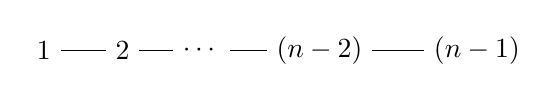
\begin{tikzpicture}
			\node (1) at (1,0) {$1$};
			\node (2) at (2,0) {$2$};
			\node (3) at (3,0) {$\cdots$};
			\node (4) at (4.5,0) {$(n-2)$};
			\node (5) at (6.5,0) {$(n-1)$};
			\draw (1) -- (2) -- (3) -- (4) -- (5);
	\end{tikzpicture}.
	\end{center}
	We will see in the exercises that the dihedral group has Coxeter diagram $\begin{tikzcd}1\ar[r,"m", no head]&2\end{tikzcd}$. 
	
	\section{Posets}
	We will be especially interested in partial orders that arise from Coxeter theory. 
	\begin{definition}
		A \newword{partial ordering} of a set $W$ is a binary relation $\leq$ which is 
		\begin{itemize}
			\item Reflexive: $x\leq x$, and
			\item Transitive: if $x \leq y$ and $y\leq z$, then $x\leq z$, and
			\item Antisymmetric: if $x \leq y$ and $y\leq x$, then $x=y$.
		\end{itemize}
		The pair $(W,\leq)$ is called a \newword{poset}.
	\end{definition}
	
	An example of a poset is the divisibility relation between positive integers. A non-example is the divisibility relation between all non-zero integers, since $1$ divides $-1$ which divides $1$, but $1\neq -1$.
	
	As usual, we write $x<y$ if $x\leq y$ and $x\neq y$. It may be possible that two elements $x$ and $y$ satisfy neither $x\leq y$ nor $y\leq x$; in this case we say that $x$ and $y$ are \newword{incomparable}. Otherwise, $x$ and $y$ are \newword{comparable}. We will depict posets using \newword{Hasse diagrams}. A Hasse diagram draws the elements of the poset so that smaller elements are below larger elements. We depict the order relations by putting an edge between two elements $x$ and $y$ if $x<y$ and there does not exist $z\in W$ such that $x<z<y$. (If this occurs, then we say that $y$ \newword{covers} $x$ or that the pair $(x,y)$ is a \newword{cover relation}.) An example is the following:
	\begin{center}
		\begin{tikzpicture}
			\node (w) at (0,0) {$w$};
			\node (x) at (-1,1) {$x$};
			\node (y) at (-1,2) {$y$};
			\node (z) at (1,1) {$z$};
			\draw (y) -- (x) -- (w) -- (z); 
		\end{tikzpicture}
	\end{center}
	This depicts a partial order on the set $\{w,x,y,z\}$. In this partial order, $w\leq x$, $w\leq y$, $w\leq z$, and $x\leq y$. The elements $y$ and $z$ are incomparable (as are $x$ and $z$). Note that we do not draw an edge between $w$ and $y$ even though $w < y$; this is because $x$ is between $w$ and $y$, so $(w,y)$ is not a cover relation.
	
	
	Let $W$ be a Coxeter group. There are two partial orderings of $W$ that are of utmost importance in applications. One is the \newword{Bruhat order}, denoted by $\leq$, and the other is the \newword{weak order}, denoted by $\leq_R$.  The name ``weak order'' is because $\leq_R$ is weaker than $\leq$, meaning that $x\leq_R y$ implies $x\leq y$. We will discuss these orders in greater detail in the remaining lectures. For now, we shall just give the definition.
	
	\begin{definition}
		Let $u,v \in W$. We say that $u\leq_R v$ if there exists a reduced word $s_{i_1}s_{i_2}\cdots s_{i_k}$ for $v$ and an index $j \in [0,k]$ such that $u = s_{i_1}s_{i_2}\cdots s_{i_j}$. We say that $u \leq v$ if there exists a reduced word for $v$ with a subword that multiplies to $u$.
	\end{definition}
	
	The Hasse diagrams for these two partial orders on $S_3$ are shown below; the weak order is shown on the left, and the Bruhat order is shown on the right.
	
	\begin{center}
		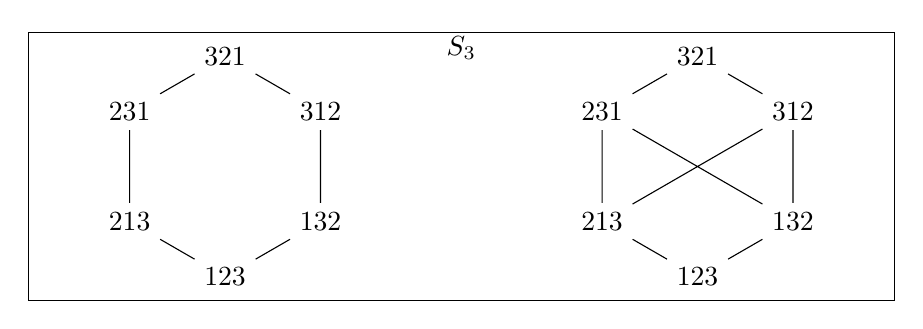
\begin{tikzpicture}[scale=1]
			\node (B) at (270:1.4) {$123$};
			\node (L1) at (210:1.4) {$213$};
			\node (L2) at (150:1.4) {$231$};
			\node (T) at (90:1.4) {$321$};
			\node (R2) at (30:1.4) {$312$};
			\node (R1) at (-30:1.4) {$132$};
			\draw (B) -- (L1) -- (L2) -- (T) -- (R2) -- (R1) -- (B);
			% \useasboundingbox (CBSW) rectangle (CBNE);
			\draw (-2.5,-1.7) rectangle (8.5,1.7);
			\node at (3,1.5) {$S_3$};
			\begin{scope}[scale=1,shift={(6,0)}]
				\node (B) at (270:1.4) {$123$};
				\node (L1) at (210:1.4) {$213$};
				\node (L2) at (150:1.4) {$231$};
				\node (T) at (90:1.4) {$321$};
				\node (R2) at (30:1.4) {$312$};
				\node (R1) at (-30:1.4) {$132$};
				\draw (B) -- (L1) -- (L2) -- (T) -- (R2) -- (R1) -- (B);
				\draw (L1) -- (R2) (R1) -- (L2);
				% \useasboundingbox (CBSW) rectangle (CBNE);
				% \draw (-2,-1.7) rectangle (2,1.7);
				% \node at (0,2) {$S_3$};
			\end{scope}
		\end{tikzpicture}
	\end{center}
	
	\section{Problems}
	
	\begin{enumerate}
		\item Warm up: compute the one-line notation of the permutation $(2,4)(2,3)(1,4)(1,3)(1,2)$ in $S_4$.
		
		\item Show that the simple transpositions generate $S_n$.
		
		\item Show that the reflections in $S_n$ are the transpositions.
		
		
		\item Show that every non-identity element of a Coxeter group has a descent. If $s$ is a descent of $w$, show that $\ell(ws)= \ell(w)-1$.
		
		\item In the following problems, feel free to use the fact that, for $a<b$, having $(a,b)\in \inv(\pi)$ means $\pi^{-1}(b)<\pi^{-1}(a)$. 
		\begin{itemize}
			\item[(a)] Compute $\inv(3412)$. What is $\ell(3412)$? 
			\item[(b)] Prove that there is a unique element in $S_n$ with maximal length. What is its length? This element is often called $w_0$. 
			\item[(c)] Prove that there is a unique reflection in $S_n$ with maximal length among reflections. What is its length?
		\end{itemize}
		
		
		\item The dihedral group $I_2(m)$ is generated by an order-$2$ reflection $s_1$ and an order-$m$ rotation $R$. Define $s_2 = s_1R$. Let $S=\{s_1,s_2\}$ and show that $(I_2(m),S)$ is a Coxeter system. Show that the Coxeter diagram is $1\overset{m}{-}2$.
		
		\item Let the group $B_n$ be defined by 
		\[ B_n \coloneqq \{\pi\mid \pi\text{ is a permutation of } \{-n,-n+1,\ldots, n-1, n\}\text{ such that $\forall i,\pi(-i)=-\pi(i)$}   \}. \]
		Define the elements $s_1 =(1,2)(-1,-2)$, $s_2=(2,3)(-2,-3)$, $\ldots,$ $s_{n-1}=(n-1,n)(-n+1,-n)$ and the element $s_0^B=(-1,1)$. Let $S = \{s_0^B,\ldots, s_{n-1}\}$. Then $(B_n,S)$ is a Coxeter system (optional exercise: prove it). 
		\begin{itemize}
		\item What is its Coxeter diagram? 
		\item How many elements are in $B_n$?
		\item How many reflections are in $B_n$?
		\end{itemize} 
		The group $B_n$ is also sometimes called $C_n$.
		
		
		\item Define a partial order on partitions of length $k$ so that $\lambda \leq \mu$ if and only if $\lambda_i\leq \mu_i$ for all $i$. 
		\begin{itemize}
		\item[(a)] Let $X$ be the set of partitions of length $2$ which are $\leq (2,2)$. (There are $6$ elements of $X$.) Draw the Hasse diagram for $X$.
		\item[(b)] Can you describe the cover relations in this partial order?
		\end{itemize}
		
		
		\item Verify that the Hasse diagrams for the weak order and Bruhat order on $S_3$ match the ones from the lecture.
		
		\item Prove that if two distinct elements of a Coxeter group have the same length, then they are incomparable in Bruhat order.
		
		
		\item There are several important properties of Coxeter groups that are all equivalent to the definition. Try proving a few from our definition:
		\begin{itemize}
			\item[(a)] Strong Exchange Property: If $t\in \inv(w)$ and $s_{i_1}\cdots s_{i_k}$ is a reduced word for $w$, then there exists a $j$ so that  $tw = s_{i_1}\cdots \widehat s_{i_j}  \cdots s_{i_k}$. (The hat notation means to omit $s_{i_j}$ from the word.)
			
			\item[(b)] Exchange Property: If $s$ is a descent of $w$ and $s_{i_1}\cdots s_{i_k}$ is a reduced word for $w$, then there exists a $j$ so that  $ws = s_{i_1}\cdots \widehat s_{i_j}  \cdots s_{i_k}$.
			
			\item[(c)] Deletion Property: If $s_{i_1}\cdots s_{i_k}$ is a non-reduced word for $w$, then there exist $j$ and $j'$ so that $w = s_{i_1}\cdots \widehat s_{i_j} \cdots \widehat s_{i_{j'}} \cdots s_{i_k}$.
		\end{itemize}
		
		
		\item Let the group $D_n$ be defined by 
		\[ D_n \coloneqq \{ \pi \in B_n \mid  \text{The size } |\{i\in [n] \mid \pi(i)<0\}| \text{ is even}  \}. \]
		Define the elements $s_1,\ldots, s_{n-1}$ as above, and define $s_0^D = (-1,2)(-2,1)$. Let $S=\{s_0^D,\ldots,s_{n-1}\}$. Then $(D_n,S)$ is a Coxeter system (optional exercise: prove it). What is its Coxeter diagram? 
		
		
		\item Let $W$ be a Coxeter group and let $w\in W$ and $t\in T$. Prove that $\ell(tw)-\ell(w)$ is odd.
		
		
		\item Let $W$ be a Coxeter group and let $t\in T$ be a reflection. Prove that $t$ has a palindromic reduced word.
		%		\noindent \textcolor{gray}{Hint: If $s_{i_1}\cdots s_{i_k} \cdots s_{i_1}$ is a palindromic reduced word for $t$, then $t$ is an inversion of $w=s_{i_1}\cdots s_{i_k}$. Can you find a candidate for $w$?  }
		
		\item Draw the Hasse diagrams for weak order and Bruhat order on $I_2(4)$.
		
		\item Prove that if $(x,y)$ is a cover relation in weak order, then $\ell(y) = \ell(x) + 1$. Do the same for Bruhat order.
		
		\item Prove that in the weak order on $W$, the number of elements which are covered by $x$ is at most the rank of $W$. Is the same true for Bruhat order?
		
		\item Prove that $B_3$ is isomorphic to the group generated by the reflective symmetries of a cube.
		
	\end{enumerate}
	
	
\end{document}